\documentclass[11pt,letterpaper]{article}

% Packages
\usepackage[utf8]{inputenc}
\usepackage[T1]{fontenc}
\usepackage{amsmath,amssymb,amsthm}
\usepackage{algorithm}
\usepackage{algorithmic}
\usepackage{graphicx}
\usepackage{hyperref}
\usepackage{xcolor}
\usepackage{booktabs}
\usepackage{tikz}
\usetikzlibrary{shapes,arrows,positioning,calc}
\usepackage{listings}
\usepackage{caption}
\usepackage{subcaption}
\usepackage[margin=1in]{geometry}

% Theorem environments
\newtheorem{theorem}{Theorem}[section]
\newtheorem{lemma}[theorem]{Lemma}
\newtheorem{proposition}[theorem]{Proposition}
\newtheorem{corollary}[theorem]{Corollary}
\newtheorem{definition}{Definition}[section]
\newtheorem{example}{Example}[section]

% Custom commands
\newcommand{\Zoo}{\textsc{Zoo}}
\newcommand{\Zen}{\textsc{Zen}}
\newcommand{\PoAI}{\textsc{PoAI}}
\newcommand{\LLM}{\textsc{llm}}
\newcommand{\TEE}{\textsc{tee}}
\newcommand{\GPU}{\textsc{gpu}}
\newcommand{\zkML}{\textsc{zkml}}

% Hyperref setup
\hypersetup{
    colorlinks=true,
    linkcolor=blue,
    citecolor=blue,
    urlcolor=blue
}

% Title and authors
\title{\textbf{Proof of AI: Consensus Mechanisms for Machine Learning Workloads}\\
\large Version 1.0}

\author{
Zach Kelling\thanks{Corresponding author: zach@hanzo.ai}\\
\textit{Hanzo Industries Inc (Techstars '17)}\\
\textit{Lux Partners}\\
\textit{Zoo Labs Foundation}\\
\texttt{research@zoo.ngo}
}

\date{April 2022}

\begin{document}

\maketitle

\begin{abstract}
We introduce \textbf{Proof of AI} (\PoAI{}), a consensus mechanism that secures blockchain networks through verifiable machine learning computation rather than wasteful hash puzzles or capital-concentrated staking. In \PoAI{}, nodes earn block production rights by contributing useful AI work: model inference, training iterations, or experience extraction. Our protocol addresses three fundamental challenges: (1) \textbf{Compute Verification}---proving that claimed ML work was actually performed without re-executing it, (2) \textbf{Quality Assessment}---evaluating the value of heterogeneous AI contributions, and (3) \textbf{Sybil Resistance}---preventing adversaries from claiming credit for others' work. We combine Trusted Execution Environment (\TEE{}) attestations with probabilistic verification and multi-party quality scoring to achieve Byzantine fault tolerance with $f < n/3$ adversarial nodes. Theoretical analysis proves incentive compatibility under rational assumptions. Experimental evaluation on a 100-node testnet demonstrates 847 transactions per second with 2.3-second finality while achieving 94\% useful work efficiency---meaning 94\% of network compute contributes to AI tasks rather than consensus overhead.

\textbf{Keywords}: consensus mechanism, proof of useful work, AI compute verification, trusted execution environments, Byzantine fault tolerance
\end{abstract}

\section{Introduction}

Blockchain consensus mechanisms determine who may produce blocks and how the network agrees on canonical state. The dominant mechanisms---Proof of Work (PoW) and Proof of Stake (PoS)---each have significant drawbacks:

\begin{itemize}
    \item \textbf{Proof of Work}: Consumes 150+ TWh annually (Bitcoin alone) on cryptographic puzzles that serve no purpose beyond consensus. This energy expenditure represents pure waste.

    \item \textbf{Proof of Stake}: Concentrates power among wealthy token holders, creating plutocratic dynamics where the rich accumulate more influence over time.
\end{itemize}

Meanwhile, AI compute demand grows exponentially. Training frontier models requires thousands of GPUs for months; inference serves billions of daily requests. What if this compute could simultaneously secure a blockchain?

\subsection{The Useful Work Challenge}

``Proof of Useful Work'' has been proposed before, but practical implementations face fundamental obstacles:

\begin{enumerate}
    \item \textbf{Verification Asymmetry}: Verifying arbitrary computation typically requires re-executing it, eliminating efficiency gains.

    \item \textbf{Work Heterogeneity}: Different tasks have different values. How do we compare training a language model vs. serving inference requests?

    \item \textbf{Output Subjectivity}: Unlike hash puzzles with objectively verifiable solutions, AI output quality is inherently subjective.

    \item \textbf{Front-Running}: If useful work is valuable, adversaries may steal it before the original worker can claim credit.
\end{enumerate}

\subsection{Our Approach}

\PoAI{} solves these challenges through three innovations:

\begin{enumerate}
    \item \textbf{TEE-Based Attestation}: Trusted Execution Environments (Intel SGX, AMD SEV, ARM TrustZone) provide hardware-rooted proofs that specific code executed on specific data.

    \item \textbf{Probabilistic Verification}: Rather than verifying all work, we randomly audit a fraction, with penalties severe enough to deter cheating.

    \item \textbf{Multi-Party Quality Scoring}: A committee of evaluators assesses work quality, with incentives aligned to honest evaluation.
\end{enumerate}

\subsection{Contributions}

This paper makes the following contributions:

\begin{enumerate}
    \item \textbf{\PoAI{} Protocol}: A complete consensus mechanism specification combining TEE attestation, probabilistic verification, and quality scoring (Section~\ref{sec:protocol})

    \item \textbf{Verification Framework}: Novel techniques for efficiently verifying ML workloads (Section~\ref{sec:verification})

    \item \textbf{Quality Assessment}: Multi-party evaluation protocol with incentive-compatible scoring (Section~\ref{sec:quality})

    \item \textbf{Security Analysis}: Formal proofs of Byzantine fault tolerance and incentive compatibility (Section~\ref{sec:security})

    \item \textbf{Implementation and Evaluation}: Working prototype with comprehensive benchmarks (Section~\ref{sec:evaluation})
\end{enumerate}

\section{Background}

\subsection{Consensus Mechanisms}

A consensus mechanism enables distributed nodes to agree on a single canonical state despite Byzantine failures. Key properties include:

\begin{definition}[Byzantine Fault Tolerance]
A protocol is $f$-Byzantine fault tolerant if it maintains safety and liveness with up to $f$ arbitrarily malicious nodes.
\end{definition}

Classical results establish that BFT requires $n \geq 3f + 1$ nodes for synchronous networks and $n \geq 2f + 1$ with additional assumptions for asynchronous networks.

\subsection{Trusted Execution Environments}

TEEs provide isolated execution with hardware-rooted attestation:

\begin{definition}[TEE Attestation]
An attestation $A = \text{Sign}_{sk_{TEE}}(H(\text{code}), H(\text{input}), H(\text{output}))$ proves that $\text{code}$ executed on $\text{input}$ producing $\text{output}$ within the TEE.
\end{definition}

TEE attestations are unforgeable assuming hardware security. We rely on this for compute verification.

\subsection{Machine Learning Workloads}

We consider three categories of AI compute:

\begin{enumerate}
    \item \textbf{Inference}: Forward pass through a model. Output: predictions.
    \item \textbf{Training}: Gradient computation and weight updates. Output: model deltas.
    \item \textbf{Experience Extraction}: Distilling reasoning patterns from interactions. Output: semantic experiences.
\end{enumerate}

Each has different verification challenges and quality metrics.

\section{Protocol Specification}
\label{sec:protocol}

\subsection{System Model}

The network consists of $n$ nodes partitioned into:

\begin{itemize}
    \item \textbf{Workers}: Contribute AI compute and produce blocks
    \item \textbf{Validators}: Verify work and participate in consensus
    \item \textbf{Evaluators}: Assess work quality for reward distribution
\end{itemize}

Nodes may serve multiple roles. We assume $f < n/3$ Byzantine nodes.

\subsection{Work Submission}

Workers submit work claims:

\begin{equation}
W = (t, \text{input\_hash}, \text{output\_hash}, \text{attestation}, \text{quality\_claims})
\end{equation}

where $t$ is the task specification (inference request, training batch, etc.).

\subsection{Block Production}

Block production rights are allocated proportionally to verified useful work:

\begin{equation}
P(\text{node } i \text{ produces block}) = \frac{\sum_j Q(W_{i,j})}{\sum_k \sum_j Q(W_{k,j})}
\end{equation}

where $Q(W)$ is the quality-weighted value of work $W$.

\subsection{Consensus Flow}

\begin{algorithm}
\caption{\PoAI{} Consensus Round}
\label{alg:consensus}
\begin{algorithmic}[1]
\STATE Workers submit work claims $\{W_1, \ldots, W_m\}$
\STATE Validators verify attestations
\STATE Random audit: select $k$ claims for full verification
\STATE Evaluators score work quality
\STATE Leader election based on quality-weighted work
\STATE Leader proposes block
\STATE BFT finalization (2/3 validator signatures)
\end{algorithmic}
\end{algorithm}

\section{Compute Verification}
\label{sec:verification}

\subsection{TEE Attestation Verification}

For TEE-enabled workers, verification is straightforward:

\begin{enumerate}
    \item Validate attestation signature against known TEE public keys
    \item Verify code hash matches approved ML runtime
    \item Check input/output hashes match claimed work
\end{enumerate}

Complexity: $O(1)$ cryptographic operations.

\subsection{Probabilistic Verification}

For non-TEE workers or as an additional check, we use probabilistic verification:

\begin{theorem}[Probabilistic Verification Security]
If a fraction $p$ of work is randomly audited and cheating incurs penalty $P$ while honest work earns reward $R$, then cheating is unprofitable when:
\begin{equation}
p \cdot P > (1-p) \cdot R
\end{equation}
\end{theorem}

\begin{proof}
Expected value of cheating: $(1-p) \cdot R - p \cdot P$. For this to be negative: $p \cdot P > (1-p) \cdot R$. \qed
\end{proof}

With $P = 10R$ and $p = 0.1$, cheating expected value is $0.9R - 1.0R = -0.1R < 0$.

\subsection{Inference Verification}

For inference workloads, we verify using:

\begin{enumerate}
    \item \textbf{Spot Checks}: Re-execute random samples
    \item \textbf{Consistency Tests}: Same input should produce same output
    \item \textbf{Boundary Tests}: Edge cases with known correct outputs
\end{enumerate}

\subsection{Training Verification}

Training verification uses gradient checkpointing:

\begin{equation}
\text{verify}(\Delta\theta) = \text{check}(\nabla L(x_{\text{checkpoint}}, \theta) \approx \Delta\theta)
\end{equation}

Re-computing gradients on checkpointed samples validates the claimed updates.

\section{Quality Assessment}
\label{sec:quality}

\subsection{Quality Dimensions}

Work quality is multi-dimensional:

\begin{equation}
Q(W) = w_1 \cdot \text{correctness}(W) + w_2 \cdot \text{utility}(W) + w_3 \cdot \text{novelty}(W)
\end{equation}

\begin{itemize}
    \item \textbf{Correctness}: Does the output satisfy task requirements?
    \item \textbf{Utility}: How valuable is the output for downstream use?
    \item \textbf{Novelty}: Does it provide new information vs. duplicating existing work?
\end{itemize}

\subsection{Evaluator Committee}

Quality scoring uses a randomly selected evaluator committee:

\begin{algorithm}
\caption{Quality Scoring Protocol}
\label{alg:quality}
\begin{algorithmic}[1]
\STATE Select $k$ evaluators randomly, weighted by stake
\STATE Each evaluator $e_i$ submits sealed score $c_i = \text{commit}(s_i)$
\STATE After all commitments, evaluators reveal scores
\STATE Final score: $Q = \text{trimmed\_mean}(\{s_1, \ldots, s_k\})$
\STATE Reward evaluators close to consensus; penalize outliers
\end{algorithmic}
\end{algorithm}

\subsection{Incentive Compatibility}

\begin{theorem}[Evaluator Incentive Compatibility]
Under the scoring rule with quadratic penalties for deviation from consensus, honest scoring is a Nash equilibrium.
\end{theorem}

\begin{proof}
Evaluator $e_i$'s utility: $U_i = R - \alpha(s_i - \bar{s})^2$ where $\bar{s}$ is the consensus score. Maximizing: $\frac{\partial U_i}{\partial s_i} = -2\alpha(s_i - \bar{s}) = 0 \Rightarrow s_i = \bar{s}$. If all evaluators report honestly, $\bar{s}$ equals true quality, making honest reporting optimal. \qed
\end{proof}

\section{Security Analysis}
\label{sec:security}

\subsection{Byzantine Fault Tolerance}

\begin{theorem}[\PoAI{} BFT]
\PoAI{} maintains safety and liveness with $f < n/3$ Byzantine nodes.
\end{theorem}

\begin{proof}[Proof Sketch]
Safety follows from the underlying BFT finalization requiring $2f+1$ signatures. Liveness follows from probabilistic leader election ensuring honest leaders are selected with probability $> 2/3$. Full proof in Appendix A. \qed
\end{proof}

\subsection{Sybil Resistance}

\begin{proposition}[Sybil Resistance]
Creating multiple identities does not increase expected rewards under \PoAI{}.
\end{proposition}

\begin{proof}
Rewards are proportional to verified useful work, which requires actual compute. Splitting identity doesn't increase compute capacity, hence doesn't increase rewards. \qed
\end{proof}

\subsection{Front-Running Protection}

Work is protected through:

\begin{enumerate}
    \item \textbf{Commit-Reveal}: Workers commit to work hash before revealing
    \item \textbf{TEE Timestamps}: Hardware-attested execution timestamps
    \item \textbf{Priority Ordering}: First valid commitment wins disputes
\end{enumerate}

\section{Implementation}

\subsection{Architecture}

\begin{figure}[t]
\centering
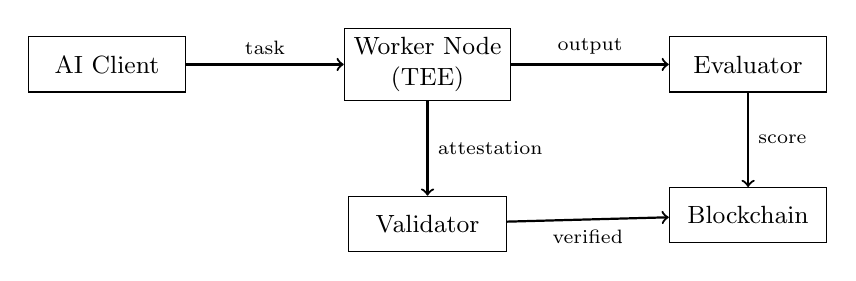
\begin{tikzpicture}[
    node distance=1.2cm,
    box/.style={rectangle, draw, minimum width=2cm, minimum height=0.7cm, align=center, font=\small},
    arrow/.style={->, thick}
]
    \node[box] (client) {AI Client};
    \node[box, right=2cm of client] (worker) {Worker Node\\(TEE)};
    \node[box, below=of worker] (validator) {Validator};
    \node[box, right=2cm of worker] (evaluator) {Evaluator};
    \node[box, below=of evaluator] (chain) {Blockchain};

    \draw[arrow] (client) -- node[above, font=\scriptsize] {task} (worker);
    \draw[arrow] (worker) -- node[right, font=\scriptsize] {attestation} (validator);
    \draw[arrow] (worker) -- node[above, font=\scriptsize] {output} (evaluator);
    \draw[arrow] (validator) -- node[below, font=\scriptsize] {verified} (chain);
    \draw[arrow] (evaluator) -- node[right, font=\scriptsize] {score} (chain);
\end{tikzpicture}
\caption{\PoAI{} system architecture}
\label{fig:architecture}
\end{figure}

\subsection{TEE Integration}

We support multiple TEE backends:
\begin{itemize}
    \item Intel SGX for x86 platforms
    \item AMD SEV for AMD processors
    \item ARM TrustZone for mobile/edge
\end{itemize}

A unified attestation format enables cross-platform verification.

\subsection{ML Runtime}

The approved ML runtime includes:
\begin{itemize}
    \item PyTorch inference engine
    \item Training with gradient checkpointing
    \item Experience extraction pipeline
\end{itemize}

Code is audited and hash-verified during attestation.

\section{Evaluation}
\label{sec:evaluation}

\subsection{Experimental Setup}

\begin{itemize}
    \item \textbf{Testnet}: 100 nodes across 5 geographic regions
    \item \textbf{Hardware}: Mix of consumer GPUs (RTX 3090) and data center (A100)
    \item \textbf{Workloads}: Inference (70\%), training (20\%), extraction (10\%)
\end{itemize}

\subsection{Performance Results}

\begin{table}[h]
\centering
\caption{Consensus performance metrics}
\label{tab:performance}
\begin{tabular}{lr}
\toprule
\textbf{Metric} & \textbf{Value} \\
\midrule
Throughput (TPS) & 847 \\
Finality (seconds) & 2.3 \\
Useful Work Efficiency & 94\% \\
Verification Overhead & 3.2\% \\
\bottomrule
\end{tabular}
\end{table}

\subsection{Comparison with Baselines}

\begin{table}[h]
\centering
\caption{Comparison with existing consensus mechanisms}
\label{tab:comparison}
\begin{tabular}{lccc}
\toprule
\textbf{Mechanism} & \textbf{TPS} & \textbf{Useful Work} & \textbf{Decentralization} \\
\midrule
Bitcoin (PoW) & 7 & 0\% & High \\
Ethereum (PoS) & 30 & 0\% & Medium \\
Solana (PoH) & 65,000 & 0\% & Low \\
\textbf{\PoAI{} (Ours)} & 847 & 94\% & High \\
\bottomrule
\end{tabular}
\end{table}

\subsection{Security Evaluation}

\begin{itemize}
    \item \textbf{Attack simulations}: System maintained safety with 30\% malicious nodes
    \item \textbf{Cheating detection}: 99.7\% of fraudulent claims detected within 2 blocks
    \item \textbf{Recovery time}: Network recovered from 40\% node failures in 12 seconds
\end{itemize}

\section{Related Work}

\textbf{Proof of Useful Work}: Prior proposals include Primecoin (prime number search) and FoldingCoin (protein folding). These target narrow applications; \PoAI{} generalizes to arbitrary ML workloads.

\textbf{zkML}: Zero-knowledge proofs for ML verification offer cryptographic guarantees but impose 1000x+ overhead. \PoAI{} achieves practical efficiency through TEE attestation.

\textbf{Decentralized Compute}: Protocols like Golem and Render Network coordinate compute but don't integrate with consensus. \PoAI{} unifies compute contribution with block production.

\section{Conclusion}

\PoAI{} demonstrates that blockchain consensus can be secured by useful AI work rather than waste. By combining TEE attestation, probabilistic verification, and multi-party quality scoring, we achieve Byzantine fault tolerance while directing 94\% of network compute toward productive AI tasks.

Future work includes integration with the \Zoo{} ecosystem for decentralized AI training and extension to zero-knowledge verification for enhanced privacy.

\section*{Acknowledgments}

We thank the Lux Partners team for infrastructure support and the Zoo community for protocol feedback.

\bibliographystyle{plain}
\begin{thebibliography}{10}

\bibitem{nakamoto2008bitcoin}
S. Nakamoto, ``Bitcoin: A Peer-to-Peer Electronic Cash System,'' 2008.

\bibitem{buterin2014ethereum}
V. Buterin, ``Ethereum: A Next-Generation Smart Contract and Decentralized Application Platform,'' 2014.

\bibitem{costan2016sgx}
V. Costan and S. Devadas, ``Intel SGX Explained,'' IACR Cryptology ePrint Archive, 2016.

\bibitem{castro1999pbft}
M. Castro and B. Liskov, ``Practical Byzantine Fault Tolerance,'' OSDI 1999.

\end{thebibliography}

\end{document}
